\documentclass[10pt,a4paper]{amsart}
\usepackage[margin=19mm]{geometry}
\usepackage{amsmath,amssymb,mathtools}
\usepackage[scr=rsfs,cal=euler]{mathalfa}
\usepackage{xfrac}
\usepackage[unicode,hidelinks,bookmarks=false]{hyperref}
\newcommand{\ie}{i.e.\ }
\newcommand{\cf}{cf.\ }
\newcommand{\resp}{respectively\ }
\newcommand{\Subsection}{\subsection}
\providecommand{\nobreakdash}{\nobreak\hbox{-}}
\setlength{\emergencystretch}{2em}
\multlinegap0pt
\usepackage{tikz}
\usepackage{amssymb}
\usepackage{mathtools}
\usepackage{xcolor}
\newtheorem{lem}{Lemma}
\title{Hochschild cohomology of the second kind:\\ Koszul duality and Morita invariance}
\author{Ai Guan, Julian Holstein, Andrey Lazarev, K. Rasmussen}
\date{Source: arXiv:2312.16645v5 (CC BY 4.0)}
\begin{document}
\maketitle

\noindent\emph{Source and licence.} Hochschild cohomology of the second kind:\\ Koszul duality and Morita invariance. Version arXiv:2312.16645v5 (CC BY 4.0), distributed by arXiv under the Creative Commons Attribution 4.0 International licence, http://creativecommons.org/licenses/by/4.0/, as recorded in the arXiv licence metadata for this exact version and shown on the abstract page https://arxiv.org/abs/2312.16645v5. Full licence notice: \texttt{licenses/arxiv-2312.16645-CC-BY-4.0.txt}.\par\smallskip

\noindent\textit{Editorial scope.} Counted unit: the article's lem lem:curved (source0.tex lines 1098--1100). The article's complete original proof of it is delivered with it (source0.tex lines 1101--1147, one \texttt{proof} environment of 47 lines). No mathematics is written, repaired or re-derived: the statement and the proof are the article's own lines, in the article's own notation, and no retained line is substituted or re-flowed.  No further source-local context is needed: every cross-reference of every retained line resolves inside the two delivered spans.  Nothing was omitted from any retained span, so the package carries no omission record.  No retained line contains a citation, so the wrapper carries no bibliography and no bibliography entry.  The retained lines contain the article's own diagram code, which the wrapper typesets with the standard tikz packages; no image file is delivered and the package declares no asset dependency.  Editorial formatting only, in addition: an AMS \texttt{amsart} preamble that restates the article's own declarations and macros used by the retained lines, namely the environments \texttt{lem} on separate counters, together with the standard packages those lines need.  The retained environments print in this document as Lemma 1 in order of appearance, whereas the article prints the same items with the numbering of its own full document.  The complete native source of the article as distributed in the arXiv e-print for this exact version is bundled unchanged as \texttt{sources/152132/source0.tex}.
\begin{lem}\label{lem:curved}
	Given a curved algebra (pc or discrete) $A=(A,d,c)$, the graded vector space $W_A$ supplied with the differential $D_c$ as above, is a curved $A$-bimodule.	Moreover, the surjective map $W_A\to A$ indiced by the multiplication map $A\otimes A\to A$, has contractible kernel. 
\end{lem}

\begin{proof}
	To show that $(W,D_c)$ is a curved $A$-bimodule we should prove that for any $x\in W_A$, it holds that $D^2_c(x)=cx-xc$. Since $W_A$ is generated, as a graded $A$-bimodule, by elements of the form $\eta(a), a\in A$ and $1\otimes 1\in A\otimes A\subset W_A$, it suffices to check the required identity for $x=\eta(a)$ or $x=1\otimes 1$.
	
	For $x=\eta(a)$, we have
	\begin{align*}
		D^2_c(x)&=D_c(i(x)-d(x))\\&=D_c(a\otimes 1-1\otimes a-\eta(da))\\
		&=[da\otimes 1-1\otimes da+a\eta(c)-\eta(c)a]-[i\eta(da))-d\eta(da)]\\
		&=[da\otimes 1-1\otimes da+a\eta(c)-\eta(c)a]-[da\otimes 1-1\otimes da-\eta(d^2a)]=\\
		&=a\eta(c)-\eta(c)a+\eta(d^2a)\\
		&=[a,\eta(c)]+\eta[c,a]\\
		&=[c,\eta(a)]
	\end{align*}
	For $x=1\otimes 1$, we have
	\begin{align*}
		D^2_c(x)&=D_c(\eta(c))\\
		&=i(\eta(c))-d\eta(c)\\
		&=c\otimes 1-1\otimes c-\eta(d(c))=\\
		&=c\otimes 1-1\otimes c.
	\end{align*}
	as required.
	
	To show that $W_A$ is weakly equivalent to $A$ as a curved $A$-bimodule, note that there is an obvious map surjective map of curved $A$-bimodules $W_A\to A$ induced by the multiplication map $A\otimes A\to A$. The kernel of this map is isomorphic to the curved $A$-bimodule having the form
	
	\[
	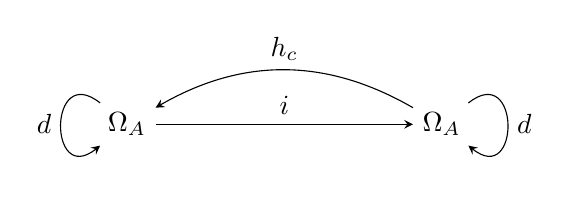
\begin{tikzpicture}[>=stealth, baseline=(current bounding box.center)]
		\node (L) at (0,0) {$\Omega_A$};
		\node (R) at (4,0) {$\Omega_A$};
		
		% straight arrow
		\draw[->] (L) -- node[above] {$i$} (R);
		
		% curved arrow right-to-left
		\draw[->] (R) to[out=150,in=30] node[above] {$h_c$}  (L);
		
		% left loop
		\draw[->]
		(L) .. controls +(-1,0.8) and +(-1,-0.8) ..
		node[left] {$d$} (L);
		
		% right loop
		\draw[->]
		(R) .. controls +(1,0.8) and +(1,-0.8) ..
		node[right] {$d$} (R);
	\end{tikzpicture}
	\]
	with $h_c$ and $i$ being mutually inverse isomorphisms. Such a curved $A$-bimodule clearly is contractible and so $W_A$ and $A$ are weakly equivalent.
\end{proof}

\end{document}
